\section{DTrace Components}

There are three main components of DTrace: the kernel module, a set of providers and the DTrace command line utility (DTrace CLI). The kernel module and providers run in kernel mode and are responsible for collecting data specified by the instrumentation and transmitting it back to userland. The DTrace CLI is the users interface to instrument the system providing the mechanisms for specifying instrumentation and displaying the results. Each component is discussed in greater detail in the following sections.

\subsection{Kernel Module}

The DTrace kernel model is the heart of the DTrace framework. This module is responsible for the coordination of all other components used in instrumentation. It keeps track of all registered providers and informs them when to enable or disable their probes. When a providers probe fires, the DTrace kernel module is responsible for executing the necessary instrumentation code and providing the data its consumers.

The kernel module is also the intermediary between the DTrace user interface and the providers. When compiling user scripts, the kernel module provides the D compiler with probe arguments and types. Once compiled, scripts are handed off to the module as Enabling Code Blocks (ECBs) to be executed as probes fire. Once executed, the data is handed back to the user interface for display to the end user.

\subsection{Provider}

Providers in DTrace provide the probe points that are used to instrument code and provide data to the end user. Dtrace includes a set of providers within the framework (see Table XXX), but developers can developer their own to expose more information from their code. These providers are often developed as separate kernel models, but there is a mechanism to allow for providers to be written for userspace processes called Userspace Defined Static Tracing (USDT). USDT is covered in Chapter XXX.

A provider is simply a collection of probe points. These probes are functions that are run when certain points of the code are reached. The probe gathers data of interest and calls back into the DTrace kernel module for further processing. Since the overhead of probes should be avoided when data is not required, the provider is responsible for tracking when probes are enables and implementing a mechanism for the kernel module to update their state.

\subsection{DTrace CLI}

The user interface to DTrace is the DTrace command line utility, DTrace(1M). Standard use of the CLI allows the user to configure DTrace parameters (such as memory usage), input scripts (either through the command line or in files) to be executed by DTrace and display the results. Other functions of the CLI are not covered in this section.

The majority of the DTrace CLI functionality is actually provided through calls to the DTrcae userspace library, libdtrace. This library is responsible for setting DTrace options, compiling D scripts, and passing compiled code to the kernel for future execution. libdtrace provides the mechanism for all interactions with DTrace in the kernel.

\section{Typical DTrace Life Cycle}

A diagram of a generic example of instrumentation with DTrace is giving in Figure \ref{fig:lifecycle}. For the purposes of this example it is assumed that the DTrace kernel module has already been loaded (usually at boot). All execution within the providers is ignored and only the interactions between components is described. Internal functions or interest within the kernel module and CLI are shown.

\begin{figure}[htpb]
	\centering
	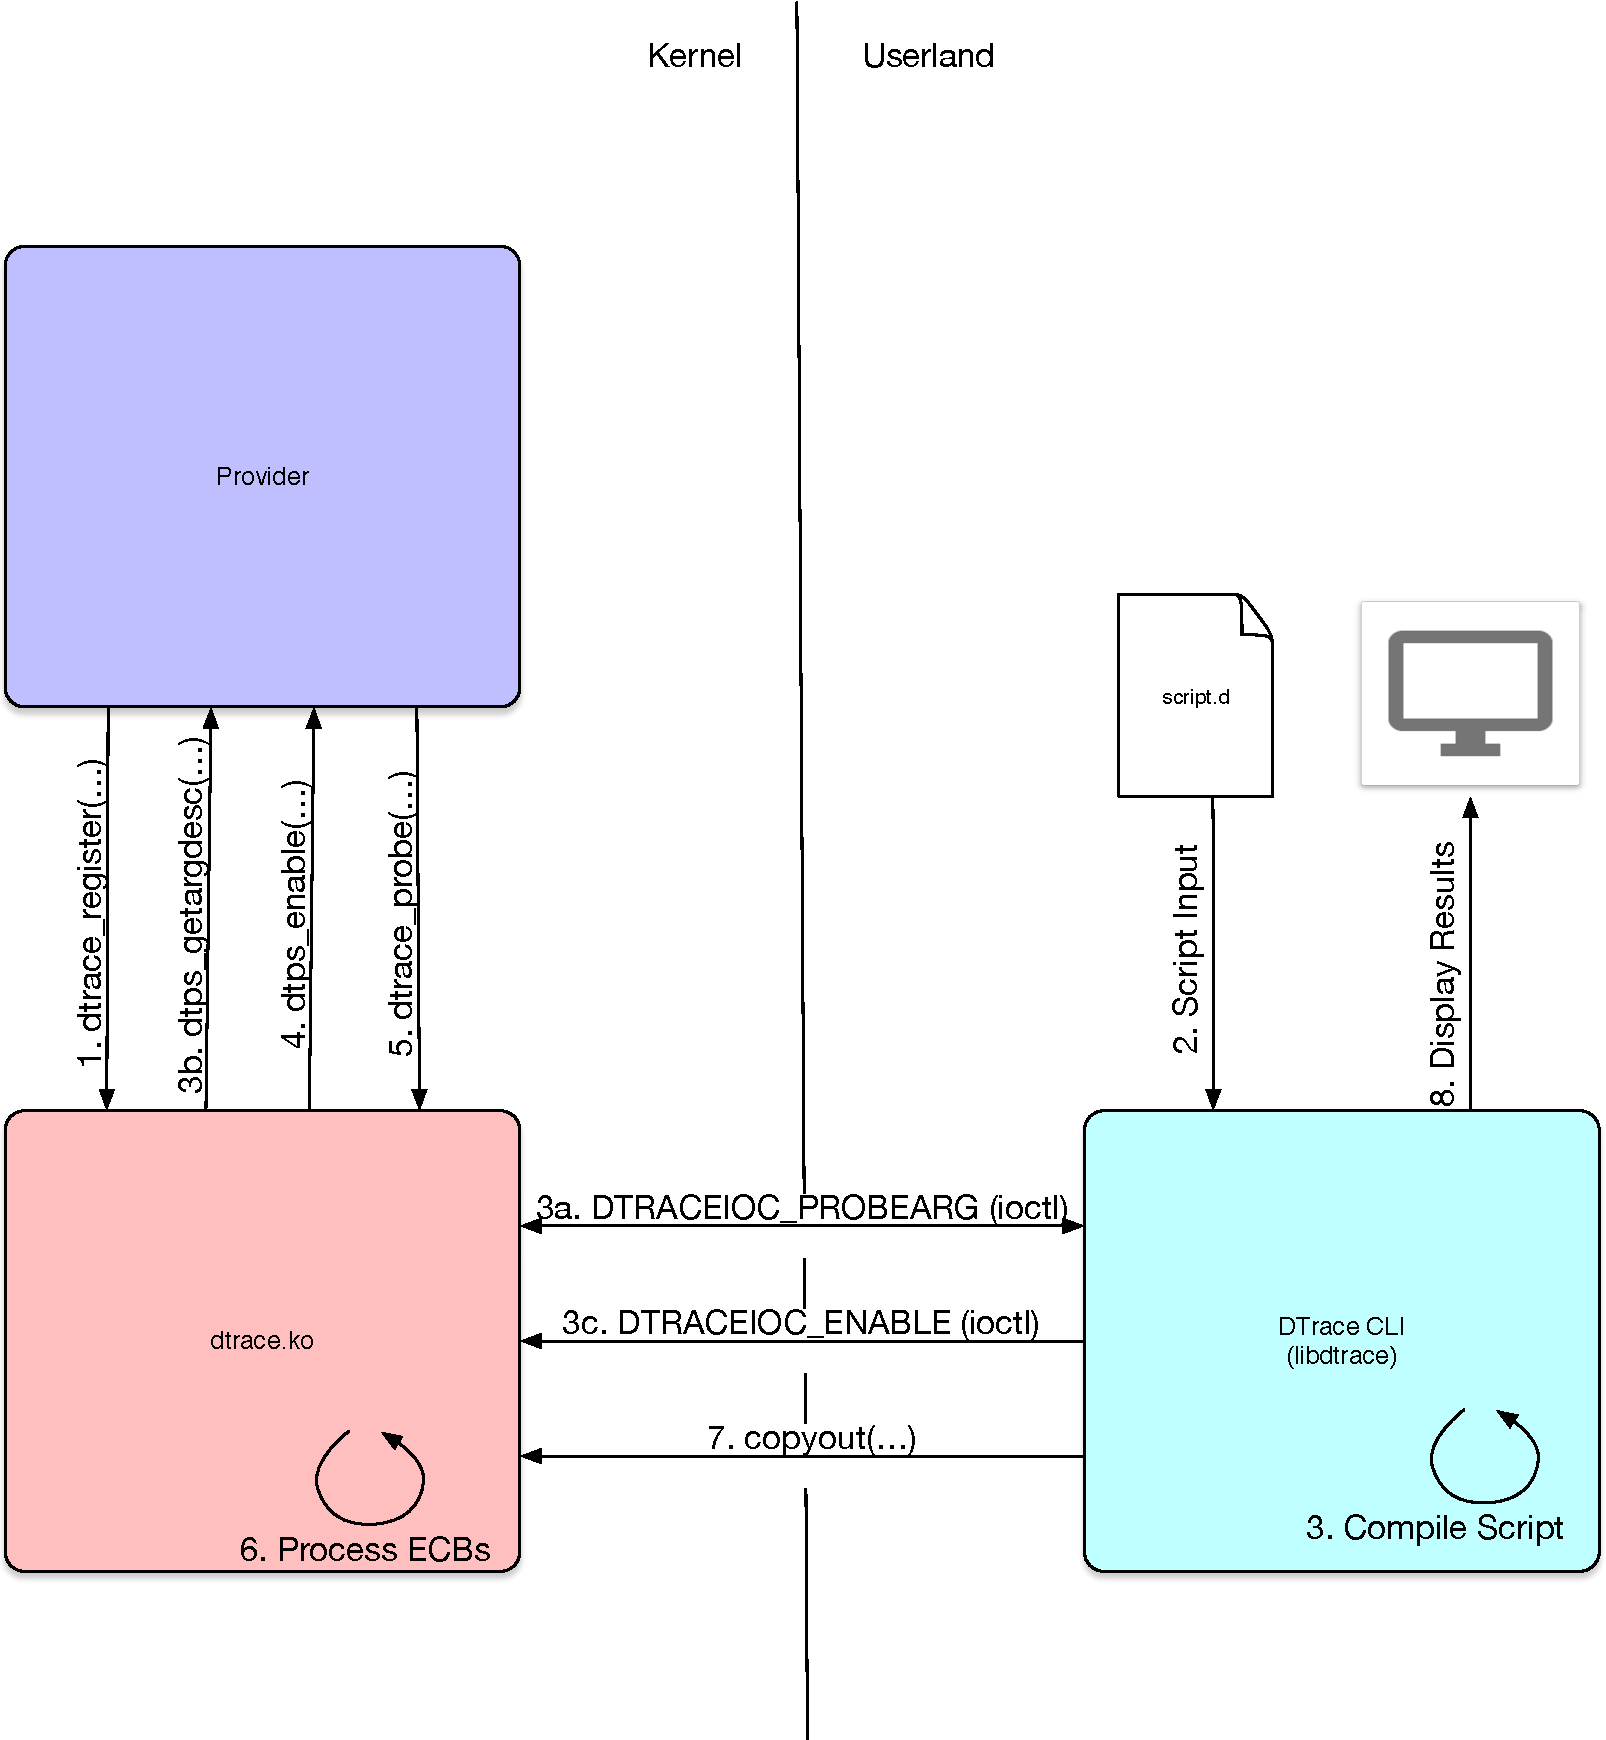
\includegraphics[width=0.8\linewidth]{dtrace-lifecycle.pdf}
	\caption{Typical lifecycle of an instrumentation using DTrace}
	\label{fig:lifecycle}
\end{figure}

When a provider is first loaded it registers itself with the DTrace kernel module (1). At this point it does enumerate all of the available probes. These probes are also disabled by default.

The provider and kernel module are then idle until such time that instrumentation is requested. This is done via the DTrace CLI, with the end user providing a D script, specifying the code to be run when a probe fires (2). When the CLI is run it initializes libdtrace, which in turn is responsible for having the kernel module initialize buffers. These buffers are used by the kernel module to store the results of the instrumentation.

libdtrace then performs the compilation of the D script (3). As part of this process the compiler queries the kernel module to determine the arguments for probes of interest via an ioctl (3a). The kernel in turn queries the provider for the probe arguments descriptions and they are returned to the compiler. In the case where probe argument types are given, the compiler can fail when there is a type mismatch. If no type information is provided the compilation will continue and any mismatch will result in a runtime error.

The result of the D script compilation is an Enabling Code Block (ECB). The ECB is provided to the kernel module (3c) which stores it with others in a tree like structure. At this point the kernel module also tell the provider to enable the probes that have been instrumented.

When a provider reaches a point in execution that has an enabled probe, it calls into the kernel module to fire it (5). The kernel module then walks through the tree of ECBs, executing any that match the probe that was fired (6). The resulting data is written into the buffer created upon the initialization of libdtrace. This data is then copied out of the kernel by the library (7). The final result are then made available to the end user (8).
